\section{Uncertainties of Measurements}
The statistic uncertainty was estimated by applying the toyMC method. 
These procedure includes 5000 iterations. In each iteration, the 'data' is filled in a 3D histogram in $X_B$-$X_C$-$recoil mass$ space. 
Then, in each bin of the histogram, the event yields fluctated according to a Poisson distribution. 
The 3D fit is applied to the fluctated 'data'. The dispersion of fitted signal event yields in signal region represents the statistic uncertainty. 
The results of toyMC test for $H\to\bpair$, $H\to\cpair$ and $H\to gg$ are represented in Fig \ref{fig:toyMC}, in terms of standard deviation of fitted signal strength. The statistic 
uncertainty of fitted signal strength for $H\to\bpair$, $H\to\cpair$ and $H\to gg$ are estimated to be 1.11\%, 10.5\% and 5.44\% respectively.
The statistic uncertainty of inclusive higgs decay is estimated in similar way, 
except for that he toyMC sample was generated by fluctuate lepton one-dimension recoil mass sepctrum, instead of three-dimension flavor-recoil mass distribution.
\begin{figure}
\label{fig:toyMC}
\centering
\subfigure[]
{ 
   \begin{minipage}[b]{0.31\textwidth}
   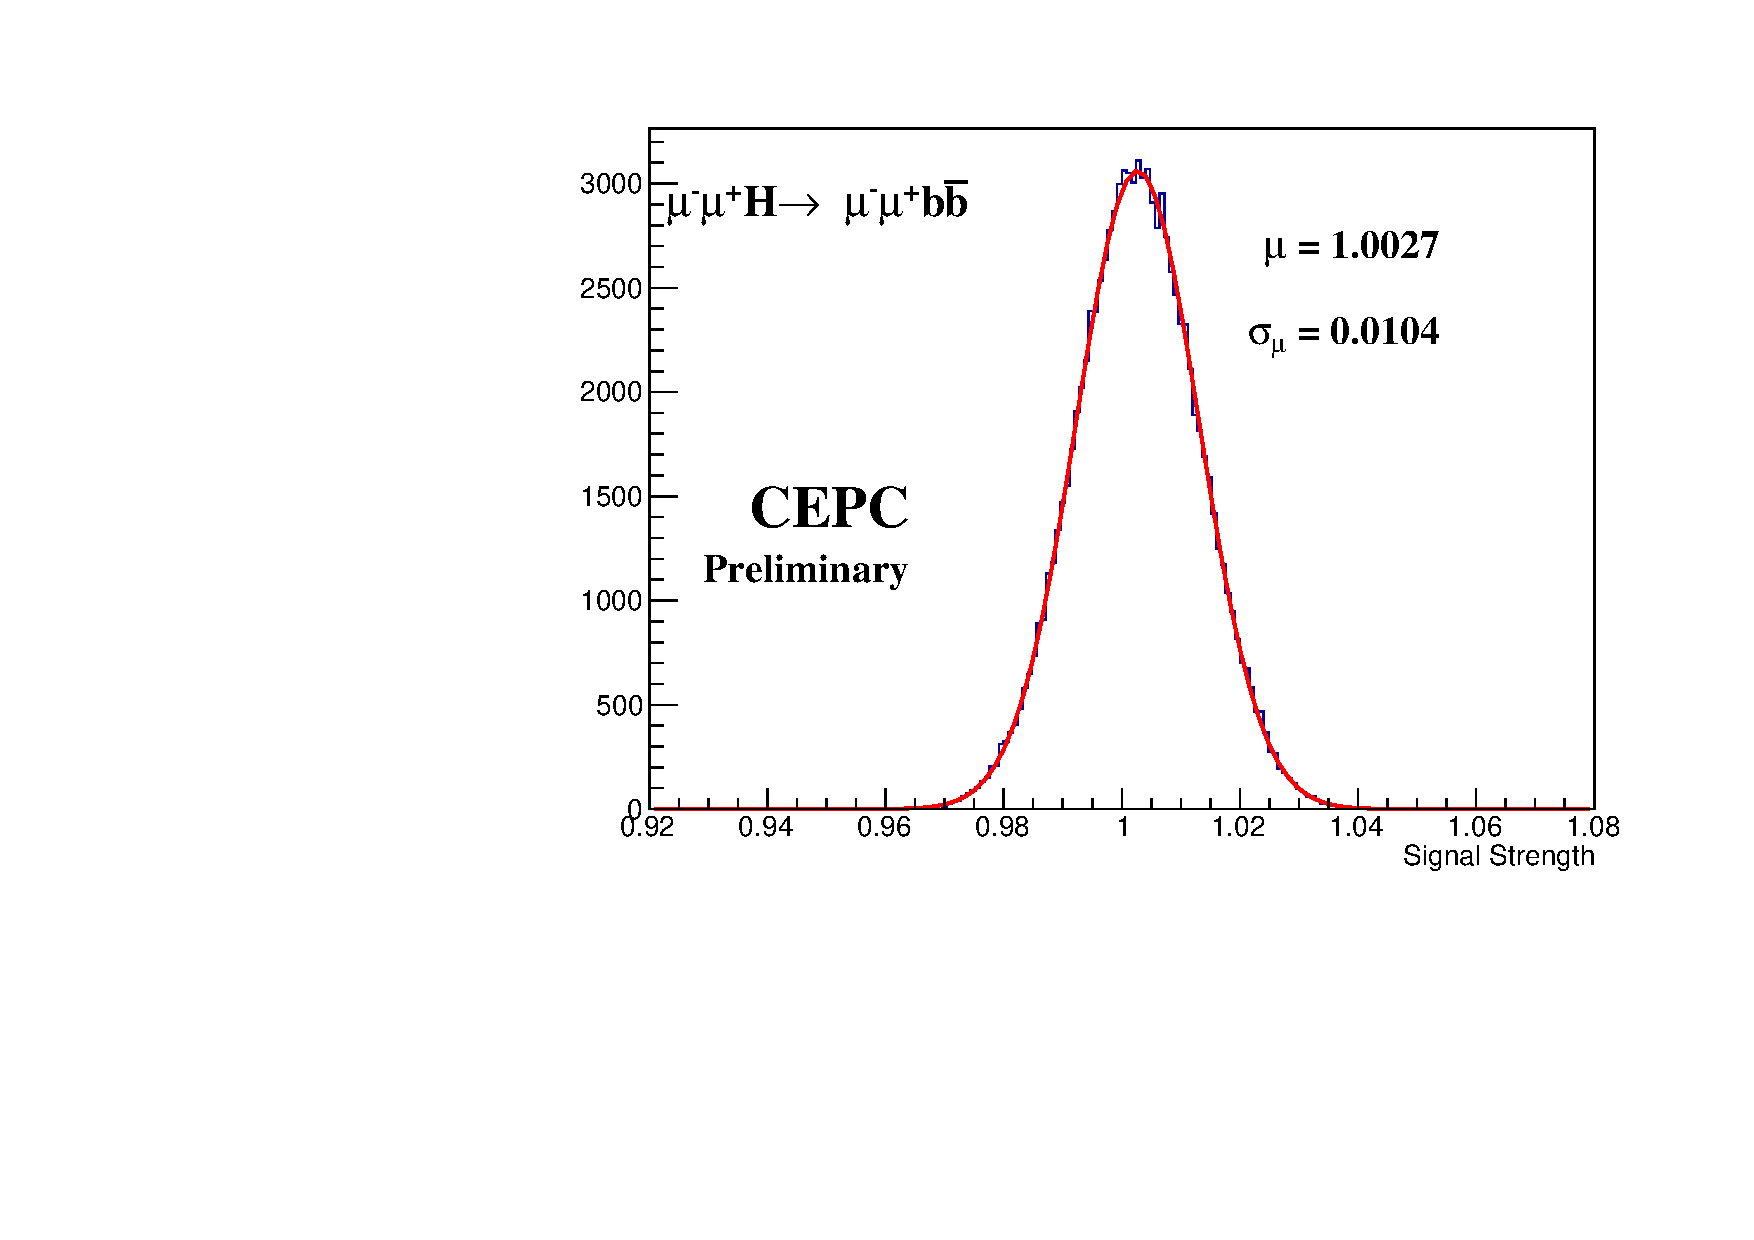
\includegraphics[width=\textwidth]{Template/toymc_mumuh_bb.pdf}
   \end{minipage}
}
\subfigure[]
{
   \begin{minipage}[b]{0.31\textwidth}
   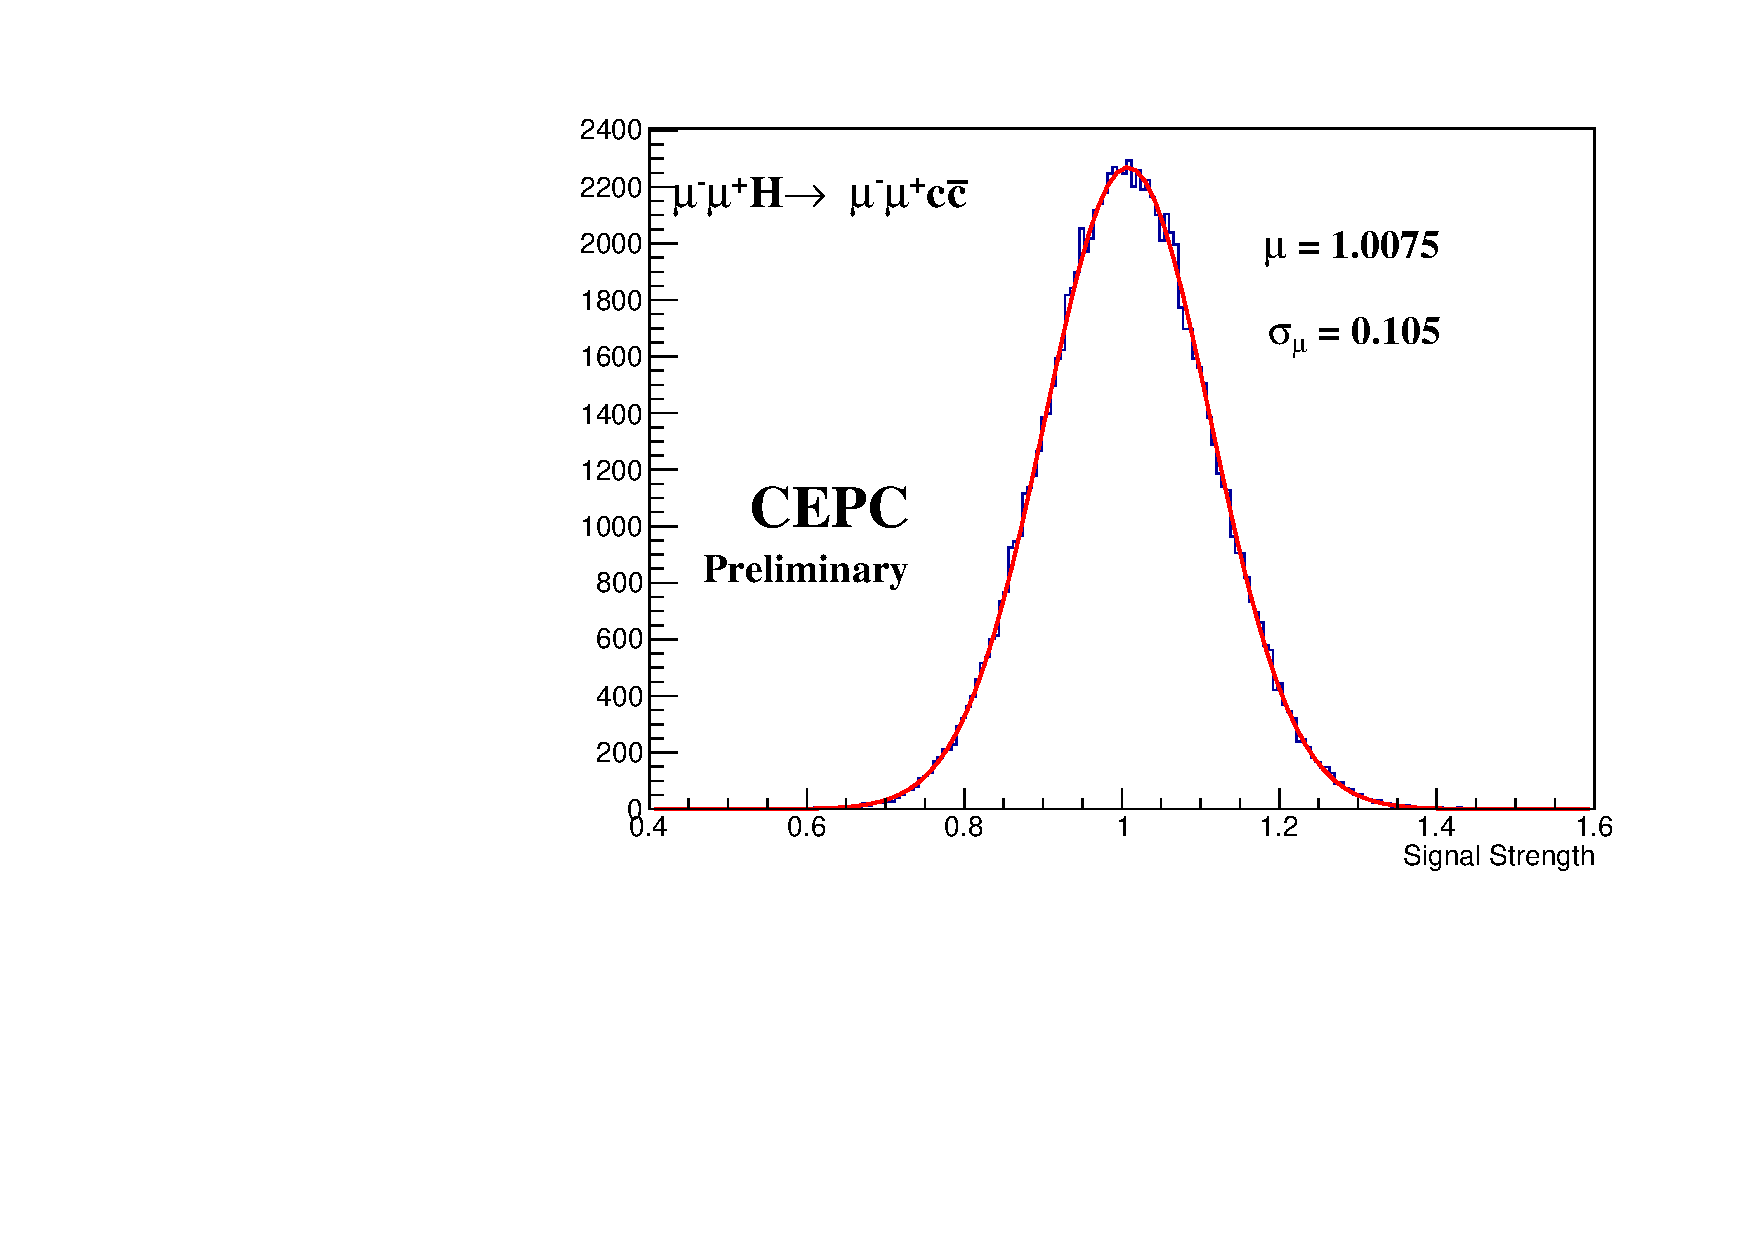
\includegraphics[width=\textwidth]{Template/toymc_mumuh_cc.pdf}
   \end{minipage}
}
\subfigure[]
{
   \begin{minipage}[b]{0.31\textwidth}
   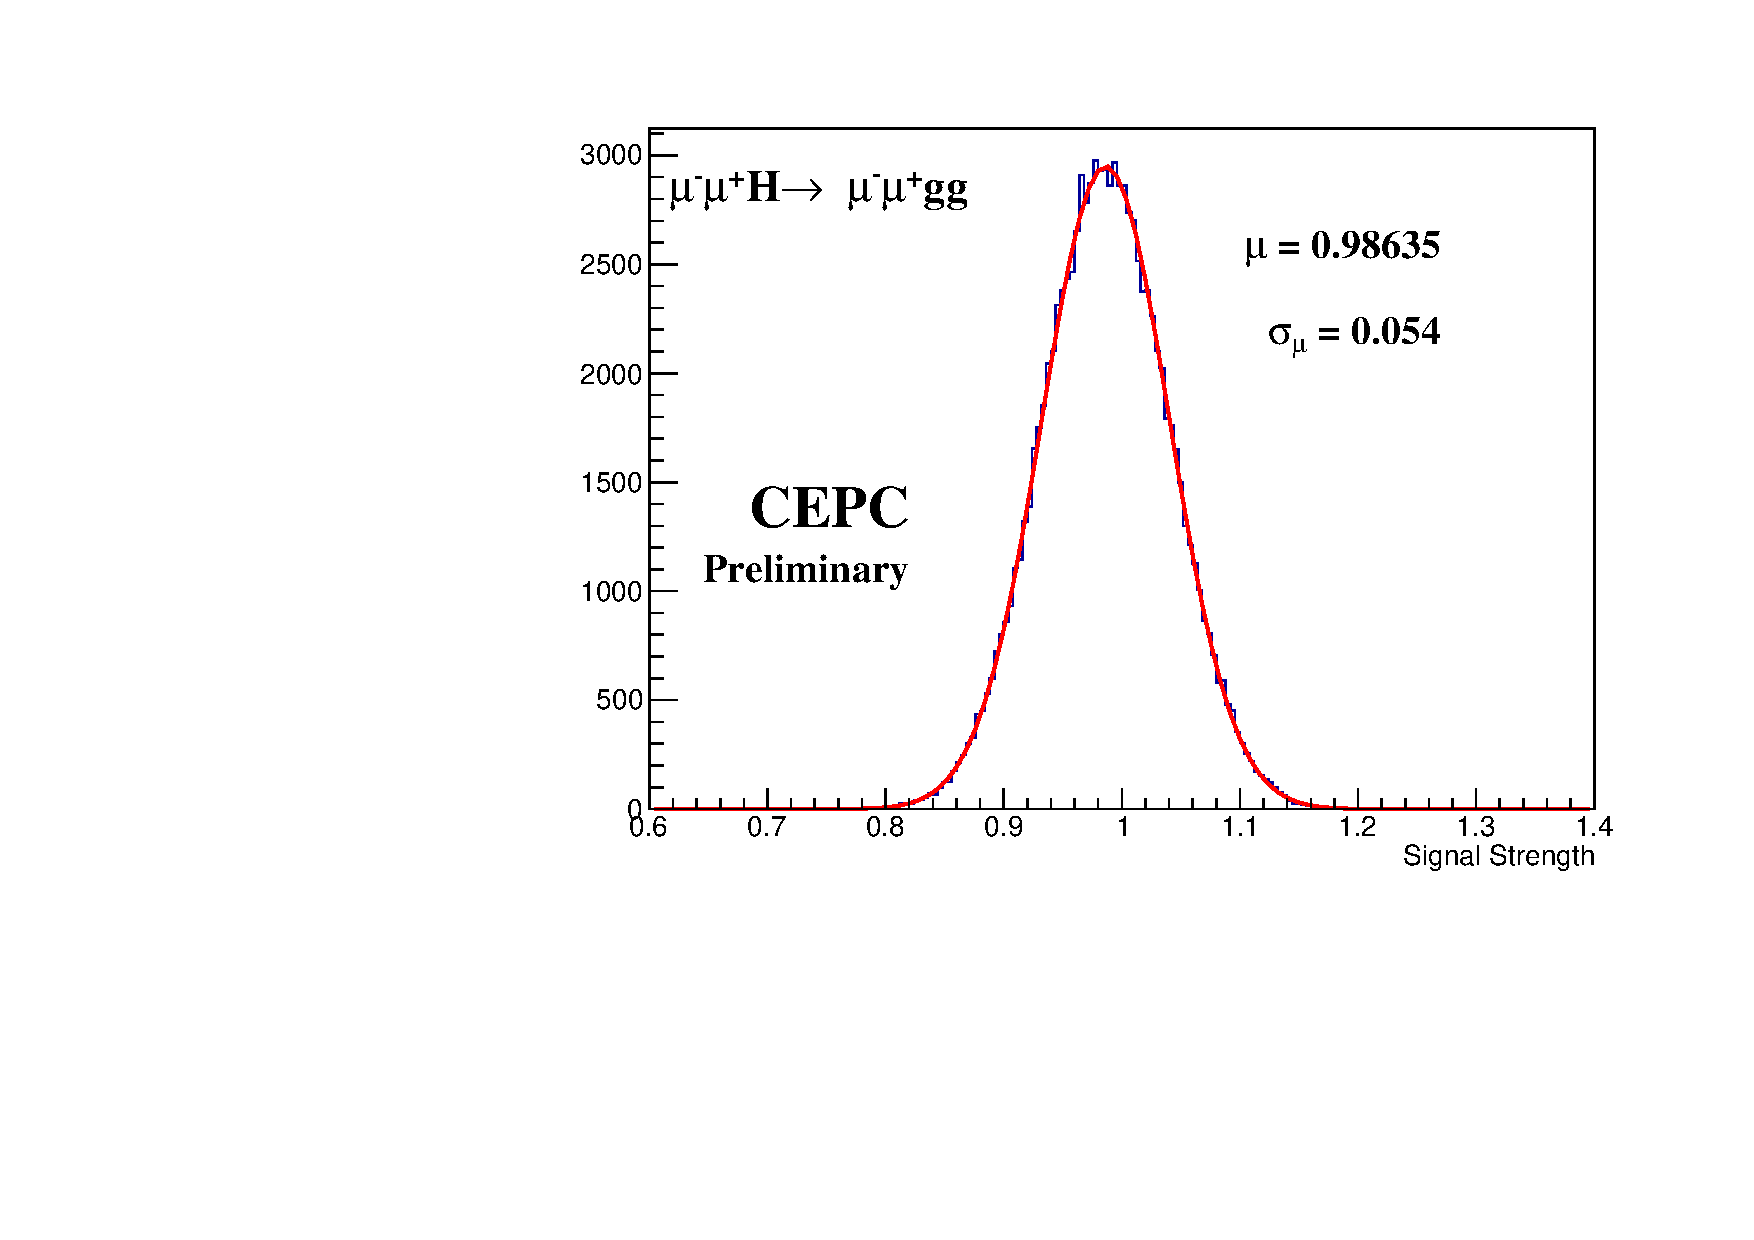
\includegraphics[width=\textwidth]{Template/toymc_mumuh_gg.pdf}
   \end{minipage}
}
\caption{Toy MC test result in terms of signal strength and uncertainty in signal region from template fit.}
\end{figure}

\par
Since the we are interested in $\dfrac{N_{H\to\bpair\cpair\gpair}}{N_{H,inclusive}}$, systematic uncertainties from lepton pair invariant mass cut, recoil 
masses cut, $Z\to\mupair$ modeling, and ISR correction canceled. Meanwhile, the signal events yields are worked out in model-indepdent way so that uncertainty from MC generator can be ignored. 
The remaining systematic sources include uncertainty from fit method, uncertainty of jet selection efficiencies, uncertainty from flavor templates and uncertainty due to non-uniformity 
in isolation lepton selection efficiency.\par
The fit method have two types of systematic uncertainty. The first kind of uncertainty is due to imperfect modeling of the PDFs. 
The PDFs include the recoil mass modeling and flavor template. The latter will be 
discussed as the systematic of flavor tagging and here we only focus on the 
recoil mass modeling.
The toyMC samples used in statistic uncertainty study are used to estimate this type of systematic uncertainty. 
The difference between the central value of fitted signal strength in toyMC test from the MC prediction are taken as the systematic uncertainty due to the modeling.\par
%By looking for the bias of fitted 
%signal events yields from that of MC prediction, we estimate the systematic uncertainty from the models in fit is 1.07\% for $H\to\bpair$, for $H\to\cpair$, for $H\to\gpair$ in $\mmh$ channel, while in $\eeh$ channel .\par
The other kind of systematic uncertainty in the fit comes from the uncertainty of we fixed parameters.
 The normalization parameters for $H\to WW^*$ 
 and $H\to ZZ^*$ backgrounds are fixed in the fit. We set these normalization parameters  5\% higher and lower to find their impact on the fitted signal yields. 
 We conservatively vary the yields of backgrounds other than $\llh$ and $ZZ\to\leppair+\qpair$ by 100\% to estimate the systematic uncertainty of fixing them.  
\par
Systematic uncertainty on lepton veto efficiency for $H\to\bpair$ can be estimate in $Z-pole$ $\bpair$ events. With one jet tagged as $b-jets$. The efficiency of lepton veto can be studied with the precision of 0.0002\% with 2 billion \bpair events in the $Z$-pole sample.
. Thus we take 0.002\% as the systematic uncertainty on lepton veto. For $H\to\cpair$ with similar method the uncertainty of lepton veto efficiency is estimated as 0.0001\%. For $H\to\gpair$ we assume the gluon jets sample yielding 1\% of that of \bpair, and estimate the 
uncertainty of lepton veto to be 0.008\%.  
The systematic uncertainties of jet PFO multiplicity, jet $\cos \theta$ cut 
and $y-$th value cut was estimated in similar way, such that by assuming these variables can be 
calibrated with the $Z-$pole sample. \par
The systematic uncertainty of the efficiency on jet pair invariant mass cut can be 
estimated from the jet energy resolution. We apply a smearing on jet pair mass distribution according to a guassian distribution corresponding to the jet energy resolution. 
We take the value of 4\% as the jet energy resolution from CEPC pre-CDR\cite{CEPC_preCDR} and get the uncertainty for $H\to \bpair$, $H\to\cpair$ and $H\to\gpair$ are $^{+0.68\%}_{-0.20\%}$, $^{+0.43\%}_{-1.08\%}$ and $^{+0.71\%}_{-1.68\%}$  respectively.\par
The systematic uncertainties due to flavor tagging are generally caused by the 
difference between templates from MC prediction and templates in data. 
To evaluate such difference, delicate flavor tagging commissioning and calibration 
are demanded. These work can be done with the $Z-pole$ data set, which include the 
quark pair production with statistics up to $~10^{10}$. The precision of flavor 
tagging commissioning will be limited by the statistic uncertainty of the 
$Z-$pole hadronic decay data set. We assume the uncertainty of the template would be 
10 times of the statistic uncertainty of the $Z-pole$ hadronic data set, and fluctuate 
the templates according to $Z-pole$ data set statistics uncertainty and fit to the dataset with fluctuated templates. The standard deviations of the fitted signal strength are taken as flavor tagging systematic uncertainty.\par

The non-uniformity of individual higgs decay channels mainly comes from leptonic or 
semi-leptonic higgs decay, which happens with diboson as intermediate states. Since 
there are extra isolation leptons, there are higher chance for these events to have 
at least two isolation leptons. On the other hand, the final states requires at 
least two particles as jet cadidiates, which will reduce the chance of leptonic process with neutrinos in the final states to pass the selection. 
Since the efficiency difference of the signal events and inclusive $\llh$ are mainly due to $H\to WW^*$ and $H\to ZZ^*$ events according to table\ref{tab:uniformity}, the uncertainty was estimated by compare the inclusive higgs efficiency with over estimated and under estimated $H\to WW^*/ZZ^*$ fraction by 5\%.\par
The systematic uncertainty estimation are summarized in table \ref{tab:systematic_uncertainties}.\par
\begin{table}
\label{tab:systematic_uncertainties}
\centering
\begin{tabular}{c|c|c|c}\hline 
             &  $H\to \bpair$ &   $H\to\cpair$    &  $H\to\gpair$    \\ \hline
   modeling  &     0.246\%    &      4.55\%       &     0.27\%       \\ \hline
 $H\to WW^*$ simulation
             & \tabincell{c}{-0.04\% \\ +0.01\%} 
                              &    \tabincell{c}{+3.7\% \\ -3.8\%}  
                                                  & \tabincell{c}{+3.9\% \\ -4.0\%} \\ \hline
 $H\to ZZ^*$ simulation       
             & \tabincell{c}{-0.02\% \\ +0.03\%}   
                              &     0.35\%        &   \tabincell{c}{-1.0\% \\ -0.83\%}\\ \hline
   other background           &   \tabincell{c}{-0.11\% \\ +0.02\%} 
                              &   \tabincell{c}{0.0\%\\ +0.9\%}
                              &   \tabincell{c}{-2.56\%\\ +2.87\%}   \\ \hline           
   extra lepton veto
             &     0.0002\%   &     0.0001\%      &    0.0008\%       \\ \hline
   Jets PFO Multiplicity    
             &     0.0001\%   &     0.0002\%      &    0.0008\%       \\ \hline
   $\cos\theta_{\mathrm{jets}}$ cut
             &     0.0006\%    &    0.0006\%      &    0.006\%        \\ \hline
   $y$ cut
             &     0.0004\%    &    0.0005\%      &    0.007\%         \\ \hline
   Jet pair mass  cut
             &  \tabincell{c}{+0.68\% \\ -0.20\%}
                              &  \tabincell{c}{+0.43\% \\ -1.08\%}
                                                  &   \tabincell{c}{+0.71\% \\ -1.68\%}\\ \hline
      \bpair  -template
             &    0.0048\%    &        0.093\%    &       0.020\%    \\ \hline 
      \cpair -template
             &    0.0016\%    &        0.056\%    &       0.021\%    \\ \hline
      \gpair  -template
             &    0.0045\%    &        0.17\%     &       0.090\%     \\ \hline
      light quark jet template
             &    0.00046\%   &       0.0076\%    &       0.0070\%    \\ \hline   
    Non uniformity
             &    \multicolumn{3}{c}{0.016\%}              \\ \hline  
  Combined   &     \tabincell{c}{+0.73\% \\ -0.36\%}
                              &  \tabincell{c}{+6.1\% \\ -6.2\%}  
                                                  &       \tabincell{c}{+7.6\% \\ -7.7\%}   \\ \hline   
 
\end{tabular} 
\caption{Systematic uncertainties of $H\to \bpair$, $H\to\cpair$ and $H\to\gpair$.}
\end{table}


%\input{texfiles/uncertainties/statistic.tex}
%\input{texfile}
